\documentclass{article}
\usepackage{graphicx}
\usepackage{siunitx}
\usepackage{booktabs}
\usepackage{caption}
\usepackage{float}
\usepackage{amsmath}
\usepackage[toc,page]{appendix}
\usepackage{breqn}


\begin{document}
\title{AP Calculus Final Project}
\author{Joshua Morin-Baxter, Alan Zhu, Nathan Wiley, and George Hong}
\date{\today}

\maketitle

\begin{abstract}
This is an analysis of data taken from the GOSH Flight Path Predictor\textsuperscript{TM}.  Four separate sets of data were analyzed: temperature vs. density, wind velocity vs. pressure, wind angle vs. wind velocity, and wind velocity vs. altitude. Each is discussed in more depth in subsequent parts.
\end{abstract}
\part{Common Tools}
For determining rates of change with discrete values, the difference quotient must be used between every point.  Define $m$ to be the average rate of change between two points.  $m$ takes the form:
$$m=\frac{\Delta y}{\Delta x}=\frac{f(x+h)-f(x)}{h}\qquad\text{First Derivative Approximation}$$
Where $h$ is the difference in value between the two values on the $x$ axis.
\\For an approximation of the second derivative, we apply the difference quotient to $m$.  Define $m^\prime$ to be:
$$m^\prime=\frac{\Delta m}{\Delta x}=\frac{m_{j+1}-m_j}{h}\qquad\text{Second Derivative Approximation}$$
Where $m_i$ are values of $m$, and $h$ is the difference in the $x$ values that return those rates of change.\\
Due to the nature of discrete data, critical points are not limited to where the first derivative is equal to zero.  The values collected are continuous, and the intermediate value theorem will apply.  When the first derivative changes signs, a critical point will also be present.
\begin{flushleft}
For this document, the term "derivative" refers to the difference quotient.
\end{flushleft}



\part{Wind Speed vs. Altitude}
A comparison of the predicted wind speed at a given altitude yields interesting trends.  Initially, the data points are closely clustered around the same windspeed (about 5\si{\frac{m}{s}}).  These are the ground conditions in the Rapid City area.  As altitude increases, however, the windspeed dips significantly before rising again - forming what appears to be a cusp (though it could possibly be a relative minimum).  This cusp behavior can be seen in Table \ref{joshtable1}: Where x=2641.95, the first derivative is negative, but at the next value recorded, x=2861.54, the first derivative has become positive.  Research~\cite{notes} indicates that this is likely a result of weather conditions near the ground, and the pressure differences that accompany them.  This relationship is explored more in Part \ref{george}.

The data is difficult to fit to any one function, but splitting it into several functions allows a reasonable model of the data.

$$
f(x) = \left\{
        \begin{array}{ll}
            t(x) & \quad 0 \leq x < 2000 \\
            h(x) & \quad 2700 \leq x < 3700 \\
            l(x) & \quad 2700 \leq x < 3680 \\
            g(x) & \quad 3680 \leq x \leq 27000
\        \end{array}
    \right.
$$

\noindent Where
\begin{align*}
  t(x) &= 2.556137318932\cdot10^{-14}x+6.44625407986886 \\
  h(x) &= -0.0069x+18.64 \\
  l(x) &= 0.0165x-41.15 \\
\end{align*} and

\begin{dmath*}
g(x) = -3.21006\cdot10^{-19}x^5 + 2.47017\cdot10^{-14}x^4 - 6.85779\cdot10^{10}x^3+ \\ 8.17467\cdot10^{-06}x^2-0.0395264x+83.9063
\end{dmath*}

This model is shown in Figure \ref{josh2}.  It helps to analyze the next notable feature of the data: a sharp change in the rate at which the wind speed is increasing.  This occurs when the altitude is approximately 5000\si{m}; After this point, the wind picks up speed at a much slower rate than before.  While $f(x)$ is not differentiable at that point of change, the derivative of points on either side lend some insight into the changing nature of the rate of increase:

\begin{align}
  l'(3679) &= 0.0165 \\
  g'(3681) &= 0.0015
\end{align}

After these initial features the most prominent pattern in the data is what appears to be an absolute maximum slightly after 10000\si{m}, before 15000\si{m}.  The graphical model $f(x)$ suggests this maximum occurs near x=11000: at this point $g'(x) = 0$ and $g''(x)$ is negative.  Wind speed increases as it approaches this maximum ($g'(x)$ is positive), though it increases at a slower and slower rate ($g''(x)$ is negative). At the maximum, the wind speed neither increases nor decreases by any significant amount ($g'(x)=0$).  After the maximum, the wind speed begins to decrease at an increasing rate ($g''(x)$ is negative).  This is the overall shape of the graph as demonstrated by Figure \ref{josh1}.  Such a dominant graphical feature is likely indicative of a comparably dominant atmospheric phenomenon, and research indicates that the largest contributor to wind speed in the upper atmosphere is the jet stream~\cite{National-Geographic}.  According to National Geographic~\cite{National-Geographic}, the Jet Stream occurs between 8 and 15 \si{km} above the earth.  This matches the data in Table \ref{joshtable1} very well.  In Part \ref{alan} the direction of the Jet Stream is determined after a similar analysis, concerning the relevance of this research.


\begin{figure}[p]
\centering
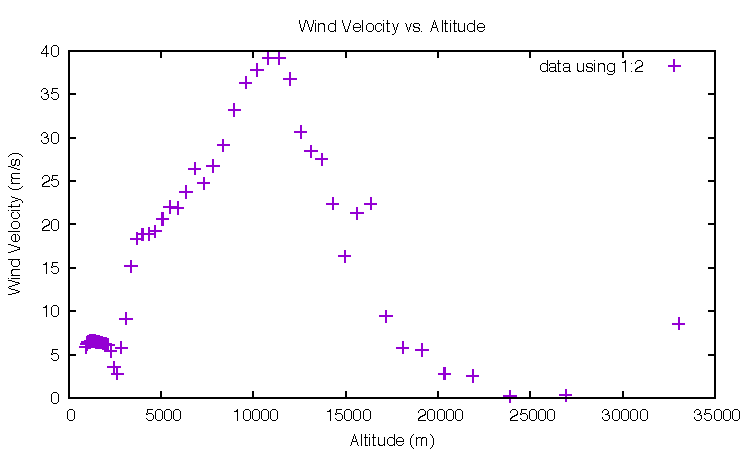
\includegraphics{josh-data/figure1.pdf}
\caption{Data comparing wind speed at various altitudes taken from the flight predictor}
\label{josh1}
\end{figure}

\begin{figure}[p]
\centering
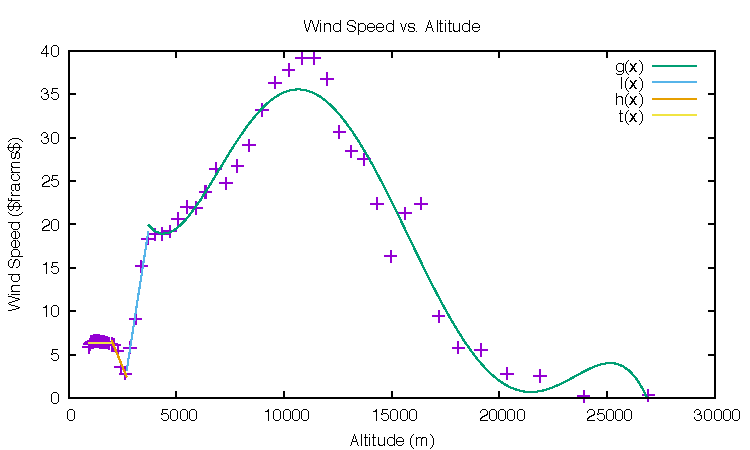
\includegraphics{josh-data/figure2.pdf}
\caption{Data plotted with line of best fit}
\label{josh2}
\end{figure}


\part{Temperature Vs. Density}

With balloon launch data, our group has picked out different variables to determine any correlation between the data and how it would make sense in the real world if there is a strong correlation between the data that we have chosen.
The data that I have chosen to analyze is temperature versus air density. In excel I have taken the first and second derivatives to get an idea of what how the two data points are related. To my knowledge right now, there is no specific pattern that the data follows; rather it is just a jumble of numbers as density, the independent variable, is decreasing.
In the data there are many points of inflection indicating a concavity change when the derivative changes from positive to negative. It is hard to analyze where the data would have these points because it jumps huge gaps between numbers when the derivative changes from positive to negative. Ergo, I am going to use the properties of calculus to determine were the regression equation:

\begin{dmath*}
   1606.69248190008x^6 + 255.343421663755x^5 + 5622.84522129159x^4 \\ -3570.2220384097x^3 + 1518.67685908935x^2 -319.719301948874x +235.092280725325
 \end{dmath*}


The data being analyzed here is temperature versus air density. In Microsoft Excel I have taken the first and second derivatives to get an idea of how the two pieces of data are related. To my knowledge, there is no specific pattern that the data follows; rather it is just a jumble of numbers as density, the independent variable, is decreasing.
Looking at the derivative data in Microsoft Excel, there are many points of inflection indicating a concavity change when the derivative changes from positive to negative--or vice versa. It is hard to analyze the data to determine exaclty where these points of inflection are because, as you can observe in the data, there are large gaps and jumps where the first derivative is a large positive value, down to very low negative values in a very short period relative to air density. Using gnu plot, I was able to plot the data and write a polynomial regression to fit the data. As you can tell by the plot, the regression calculation was success as the curve fits better than I have expected. This regression equation condenses the data I am analyzing

\begin{dmath*}
  1606.69248190008x^6 + 255.343421663755x^5 + 5622.84522129159x^4 -3570.2220384097x^3 + 1518.67685908935x^2 -319.719301948874x +235.092280725325
\end{dmath*}

Using this equation, we can find the first derivative and second derivative equations and then evaluate them to further understand our areas of interest in the excel spreadsheet data.
First derivative equation: $9640.1544x^5 + 1276.7160x^4 + 22491.3808x^3 – 10710.6660x^2 + 3037.3536x – 319.7193$
Second derivative equation: $48200.7720x^4 + 5106.8640x^3 + 67474.1424x^2 – 21421.3320x + 3037.3536$
We will find what we need using the second derivative. Specifically, what we are looking for is the possibility of the regression line having points of inflection between 0.14 and 0.3.
Temperature Density can be modeled by the equation Int|f(x) dp where f(x) is the regression line. The relationship between temperature and density gives us the product of Temperature Density which increases forever past a certain point of the graph; much like particle motion.

I was able to fit a twentieth power polynomial, tenth polynomial, and a hectic polynomial; they all fit very well with the data but fitting a very high power polynomial is not good in the sense that you can over fit the line. But at this point I’m feeling the need to quench my thirst for hardcore mathematics.

\begin{figure}[p]
\centering
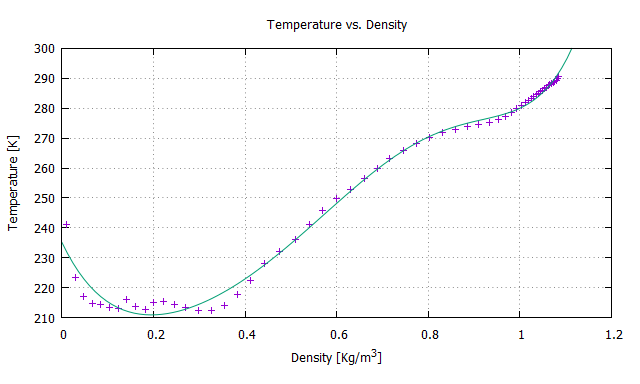
\includegraphics[scale=0.5]{nate-data/six}
\caption{Sixth Power regression line}
\label{nate1}
\end{figure}

\begin{figure}[p]
\centering
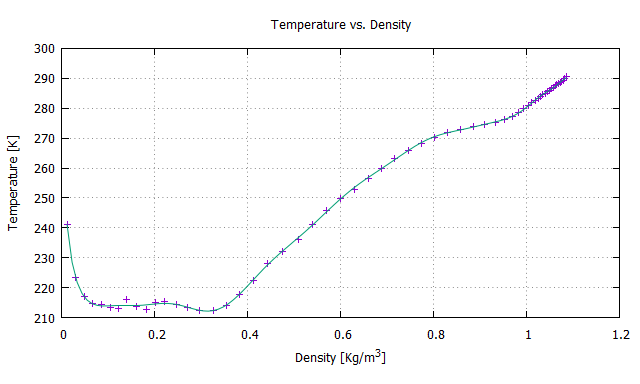
\includegraphics[scale=0.5]{nate-data/twenty}
\caption{Twentieth Power regression line}
\label{nate2}
\end{figure}

In the data, there is an interesting trend of positive and negative derivative values. This is between 0.14 and 0.3. The zeros I had found with the derivative do not fall between 0.14 and 0.3. This means that there is no maximum for the section of data I am looking at even though that the pattern indicates that there should be. There is only one point of inflection in the interval that I am looking at and is insignificant in the context of the data.
The graph fits the data very nicely but it does not tell us anything significant about the trends in the data as it is concave up and increasing most of the time during this interval.
The integrals for the derivatives effectively reverse the second derivative to the first derivative and the first derivative to the original function. The integral for the function gives you a product of temperature density.






\part{Wind Velocity vs. Pressure}
\label{george}


\begin{figure}[H]
\centering
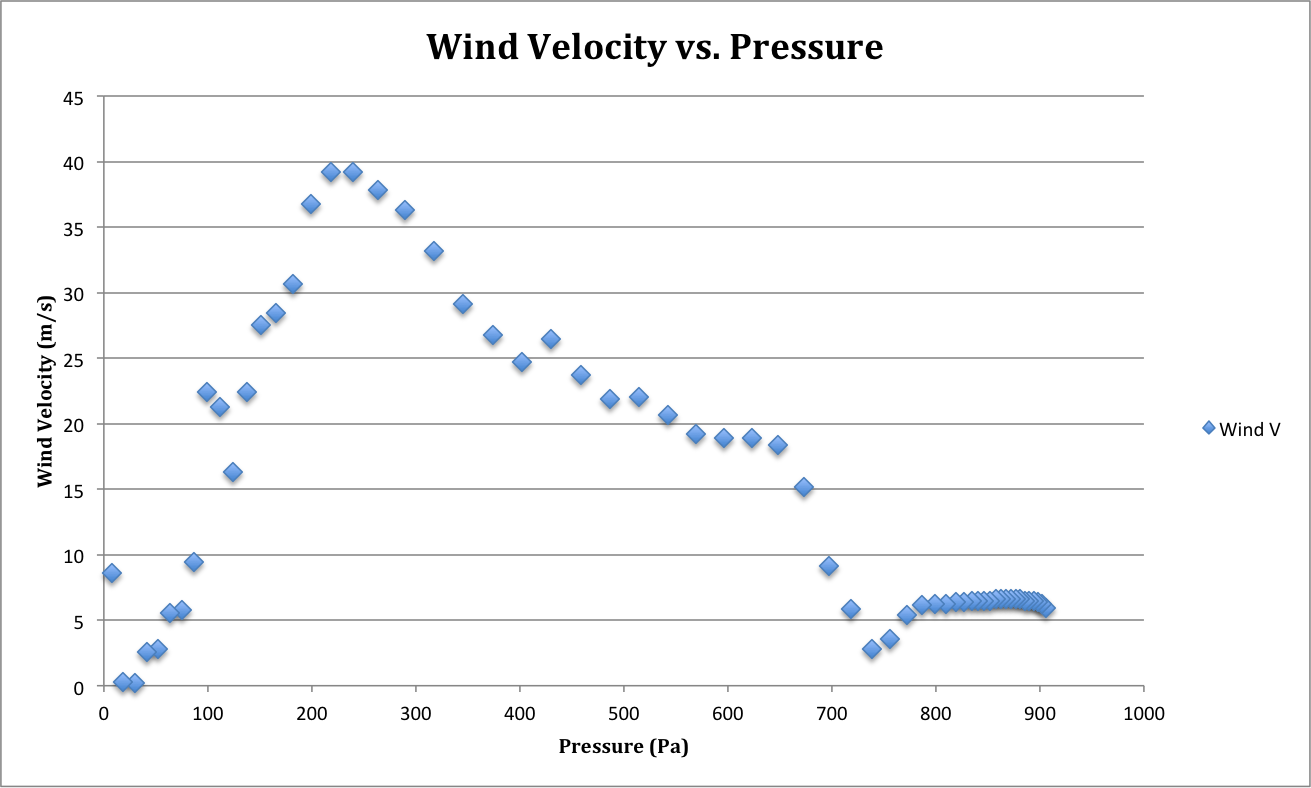
\includegraphics[width=\textwidth]{IMG1CDATA.png}
\caption{Plot of Wind Velocity vs. Pressure}
\end{figure}

\begin{flushleft}
\textbf{Analysis:} After plotting all the points in a scatterplot, we notice our predicted concavities are well matched (see Numerical Analysis of Wind Velocity vs. Pressure in the Appendix).  From the first derivative, we can split the data points into two distinct sections.  Pressures $\in$ [0,230) experience mostly increasing wind velocity, and Pressures $\in$ (230,725] experience primarily decreasing wind velocity.  Following a pressure of 800 Pascals, wind velocity stabilizes at $6.3\frac{m}{s} \pm 0.2\frac{m}{s}$.  We notice that wind speed is caused by shifts from high to low pressures, and the data from (230, 900) conforms to this principle: Wind speed increases as Pressure decreases.  Factors including temperature and the location of Jet Streams will result in divergence from this pattern.  Pressure is highest when altitude is lower, so the stable plateau of wind velocity at the highest pressures is expected.  Pressure collected in our data monotonically decreased with altitude.  Plots of Wind Velocity vs. Pressure or Altitude will resemble a horizontal reflection in this case although certain intervals will expand or contract.
\end{flushleft}

\begin{figure}[H]
\centering
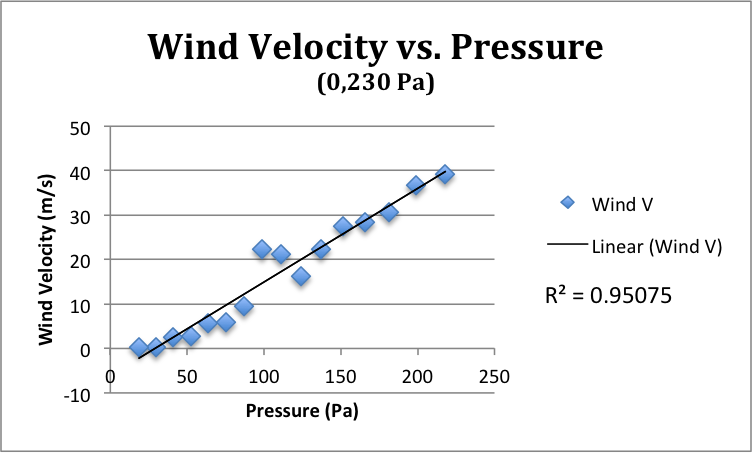
\includegraphics[width=2.25in]{LPANDA.png}\hfill 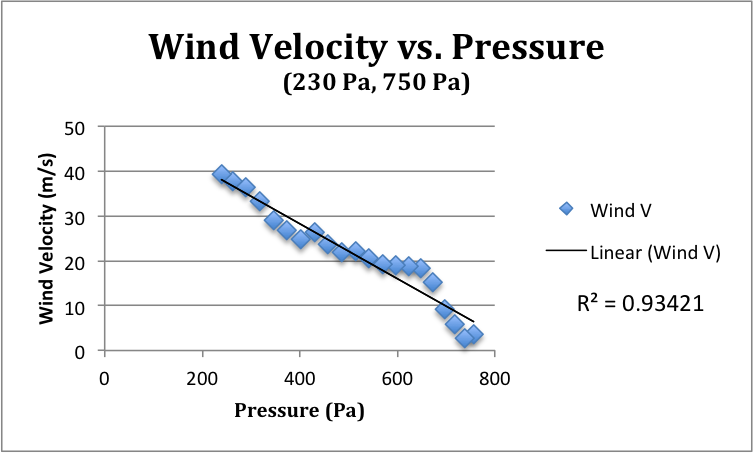
\includegraphics[width=2.25in]{RPANDA.png}
\caption{Plots of Wind Velocity vs. Pressure on Given Intervals}
\end{figure}

\begin{flushleft}
\textbf{Interpolation:} After separating the data into the intervals of (0,230) and (230,725), each plot can be fitted with a linear trend line.  Behavior within these intervals is remarkably consistent, and wind velocity can be estimated with the following equations:
\end{flushleft}

\begin{align*}
\centering
    V(P) &= 0.2107P - 6.1117&& \text{\quad $P\in(0,230)$} \\
    V(P) &= -0.0613P + 52.754 && \text{\quad $P\in(230,725)$} \\
\end{align*}



\part{Wind Velocity vs. Wind Angle}
\label{alan}

\begin{figure}[H]
  \centering
  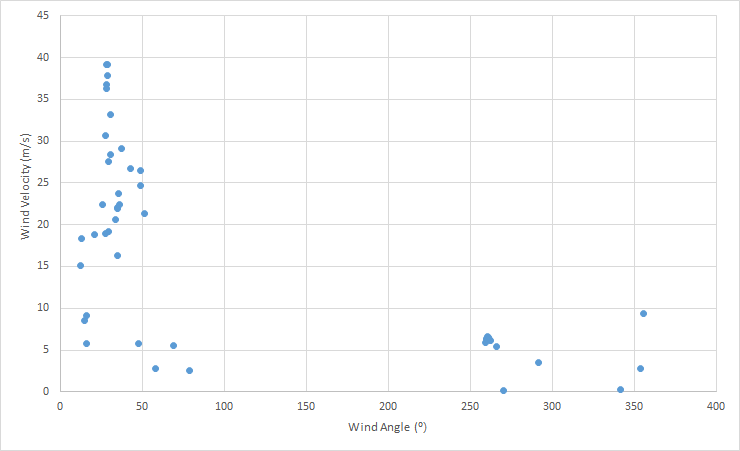
\includegraphics[width=\textwidth]{alan-data.png}
  \caption{Plot of Wind Velocity vs. Wind Angle}
\end{figure}

Although the tendencies of the data tend to wary between points, some overarching trends can be noted by analyzing the sign of the first and second derivatives (especially where they change).
The data can be analyzed on various intervals.
\begin{itemize}
  \item $\theta \in (12^{\circ},16^{\circ})$: Data varies wildly.
  \item $\theta \in (20^{\circ}, 28^{\circ})$ Data is almost consistently increasing, before reaching a critical point while being concave down (thus being a local maximum).
  \item $\theta \in (29^{\circ}, 35^{\circ})$ Data is also almost consistently increasing.
  \item $\theta \in (35^{\circ}, 37^{\circ})$ Data varies before reaching a critical point while being concave down (thus being a local maximum).
  \item $\theta \in (37^{\circ}, 48^{\circ})$ Data slowly and inconsistently decreases.
  \item $\theta \in (48^{\circ}, 52^{\circ})$ Decreases before reaching a critical point and point of inflection (thus being a local minimum).
  \item $\theta \in (53^{\circ}, 80^{\circ})$ Data varies.
  \item $\theta \in (259^{\circ}, 260.2^{\circ})$ Data is increasing and concave up before reaching a point of inflection.
  \item $\theta \in (260.2^{\circ}, 261^{\circ})$ Data is varying, but is critical and has a varying second derivative, meaning the data has a local maximum in this area.
  \item $\theta \in (261^{\circ}, 271^{\circ})$ Data is decreasing, but second derivative goes from negative to positive, reaching a critical point where the second derivative is positive (thus being a local minimum).
  \item $\theta \in (290^{\circ}, 355^{\circ})$ Data is consistently increasing, reaching a maximum at the end of the data.
\end{itemize}

The critical points on the interval $(26^{\circ}, 37^{\circ})$ and the general clustering of data around them represents the jet stream, blowing towards the NEbN (Northeast by North), while the critical point near 260 degrees seems to be the surface wind, which blows towards WbS (West by South).

The jet stream data can be fit by a normal distribution with $R = 0.536$.

\begin{figure}[H]
  \centering
  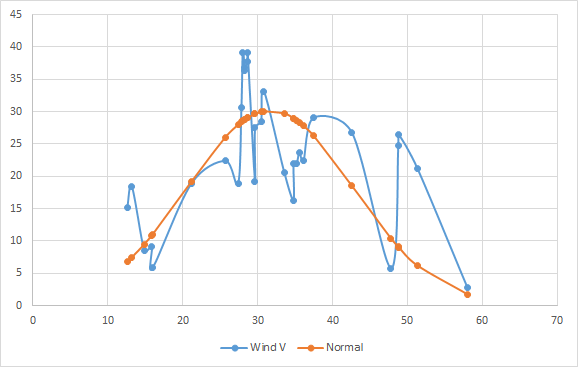
\includegraphics[width=\textwidth]{alan-data-2.png}
  \caption{Plot of Wind Velocity vs. Wind Angle on the Interval $(10^{\circ}, 60^{\circ})$ Fit by a Normal Distribution}
\end{figure}


The equation for the distribution is:
\[
wind(\theta) = \frac{1}{\sqrt{2*(11.18753)^2*\pi}}*e^{-\frac{(\theta-31.65742)^2}{2*(11.18753)^2}}*846
\]

This gives us that the mean direction of the jet stream occurs at 31.65742 degrees.




\begin{thebibliography}{1}

\bibitem{notes} John W. Dower {\em Readings compiled for History
21.479.}  1991.

\bibitem{impj}  The Japan Reader {\em Imperial Japan 1800-1945} 1973:
Random House, N.Y.

\bibitem{National-Geographic} E. H. Norman {\em Japan's emergence as a modern
state} 1940: International Secretariat, Institute of Pacific
Relations. https://www.nationalgeographic.org/encyclopedia/jet-stream/

\bibitem{fo} Bob Tadashi Wakabayashi {\em Anti-Foreignism and Western
Learning in Early-Modern Japan} 1986: Harvard University Press.

\end{thebibliography}



\appendix
\section{Charts and Graphs}

\begin{table}[H]
\centering
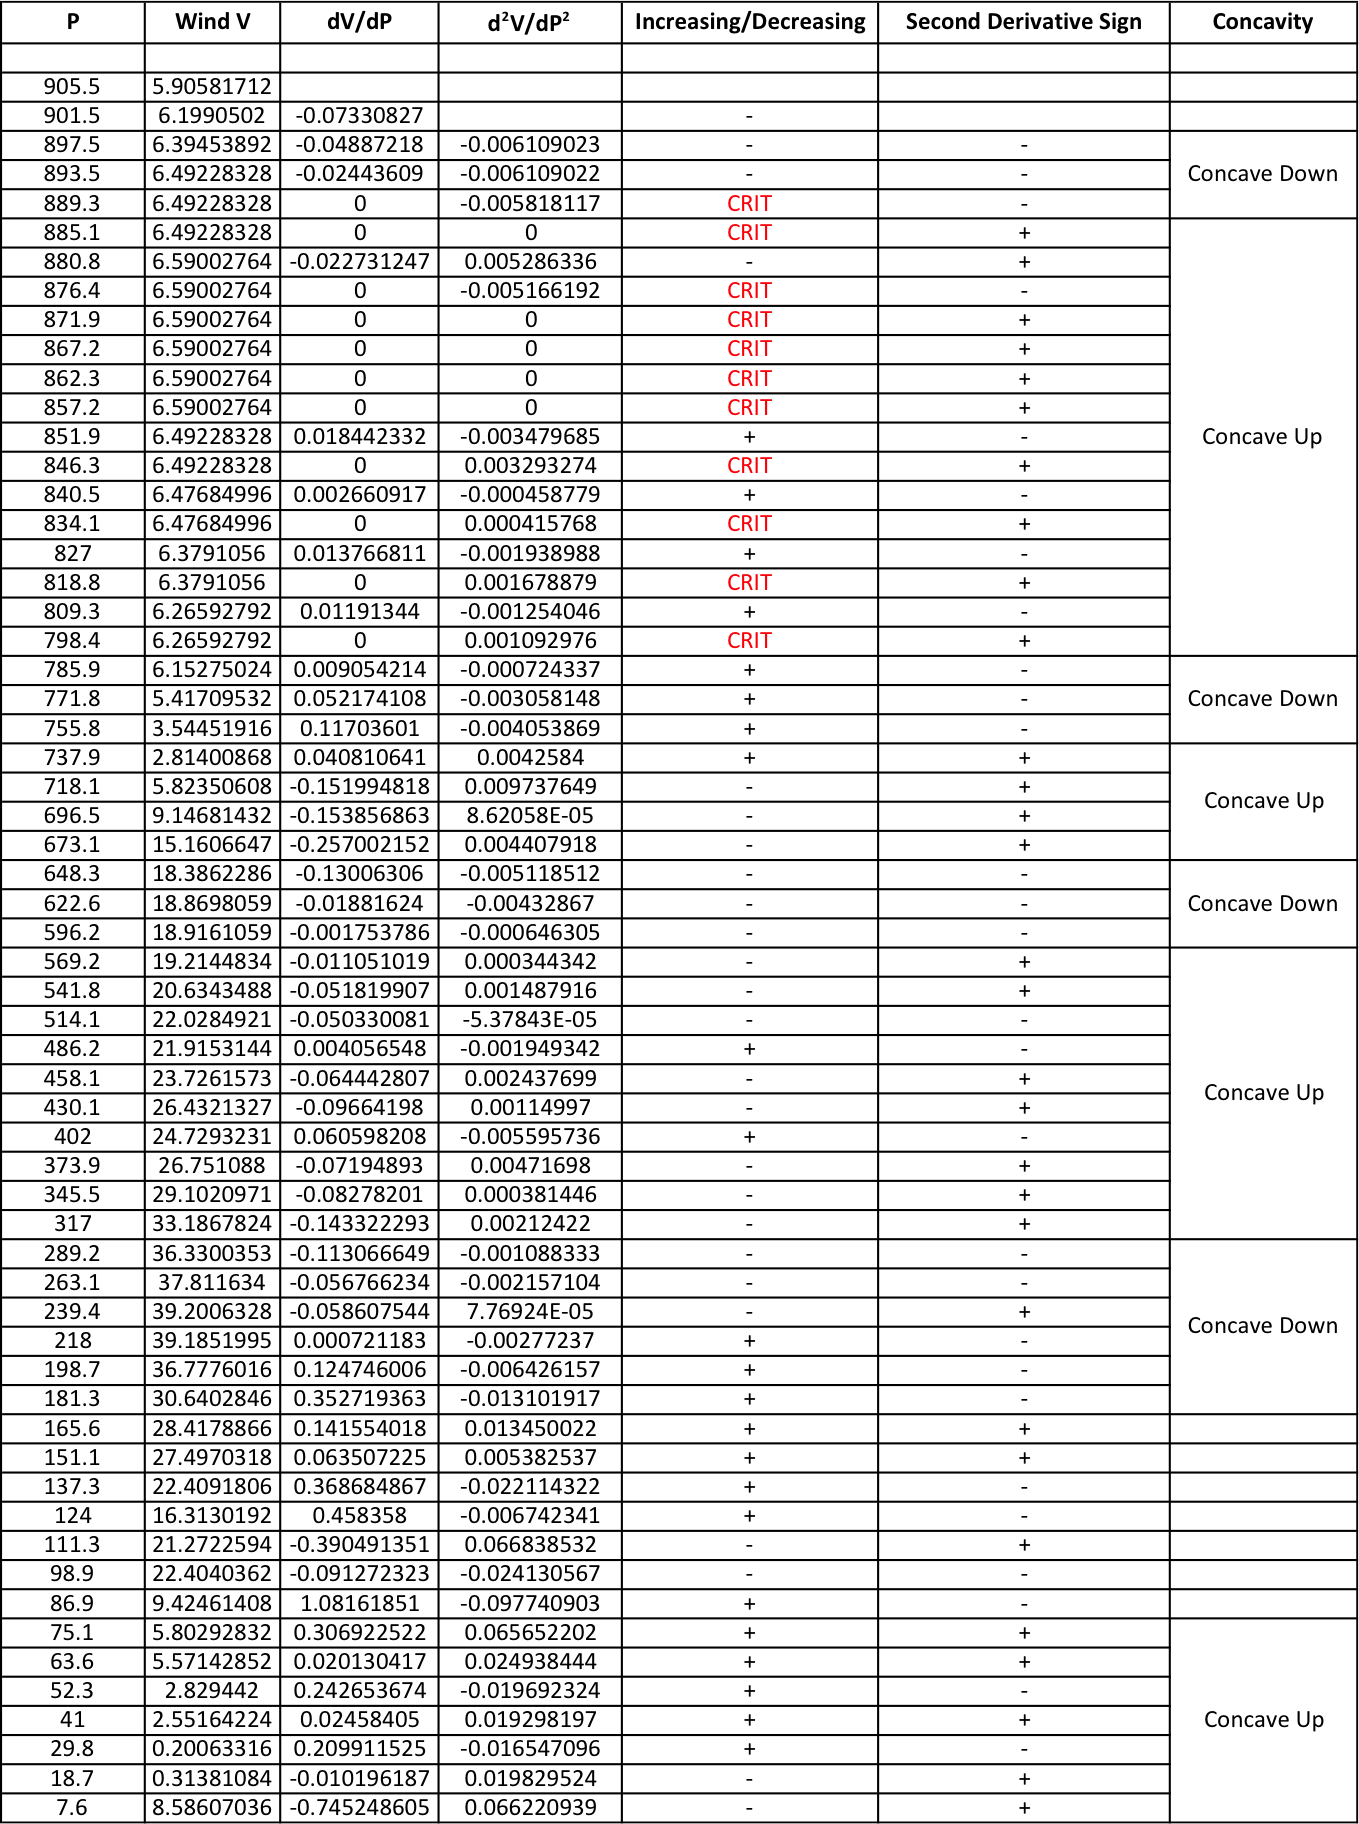
\includegraphics[width=\textwidth]{PANDA.png}
\caption{Numerical Analysis of Wind Velocity vs. Pressure.\\\textbf{Note:} Pressure monotonically decreases, so no derivative is given for the highest value of pressure.}
\end{table}

\begin{table}[H]
\centering
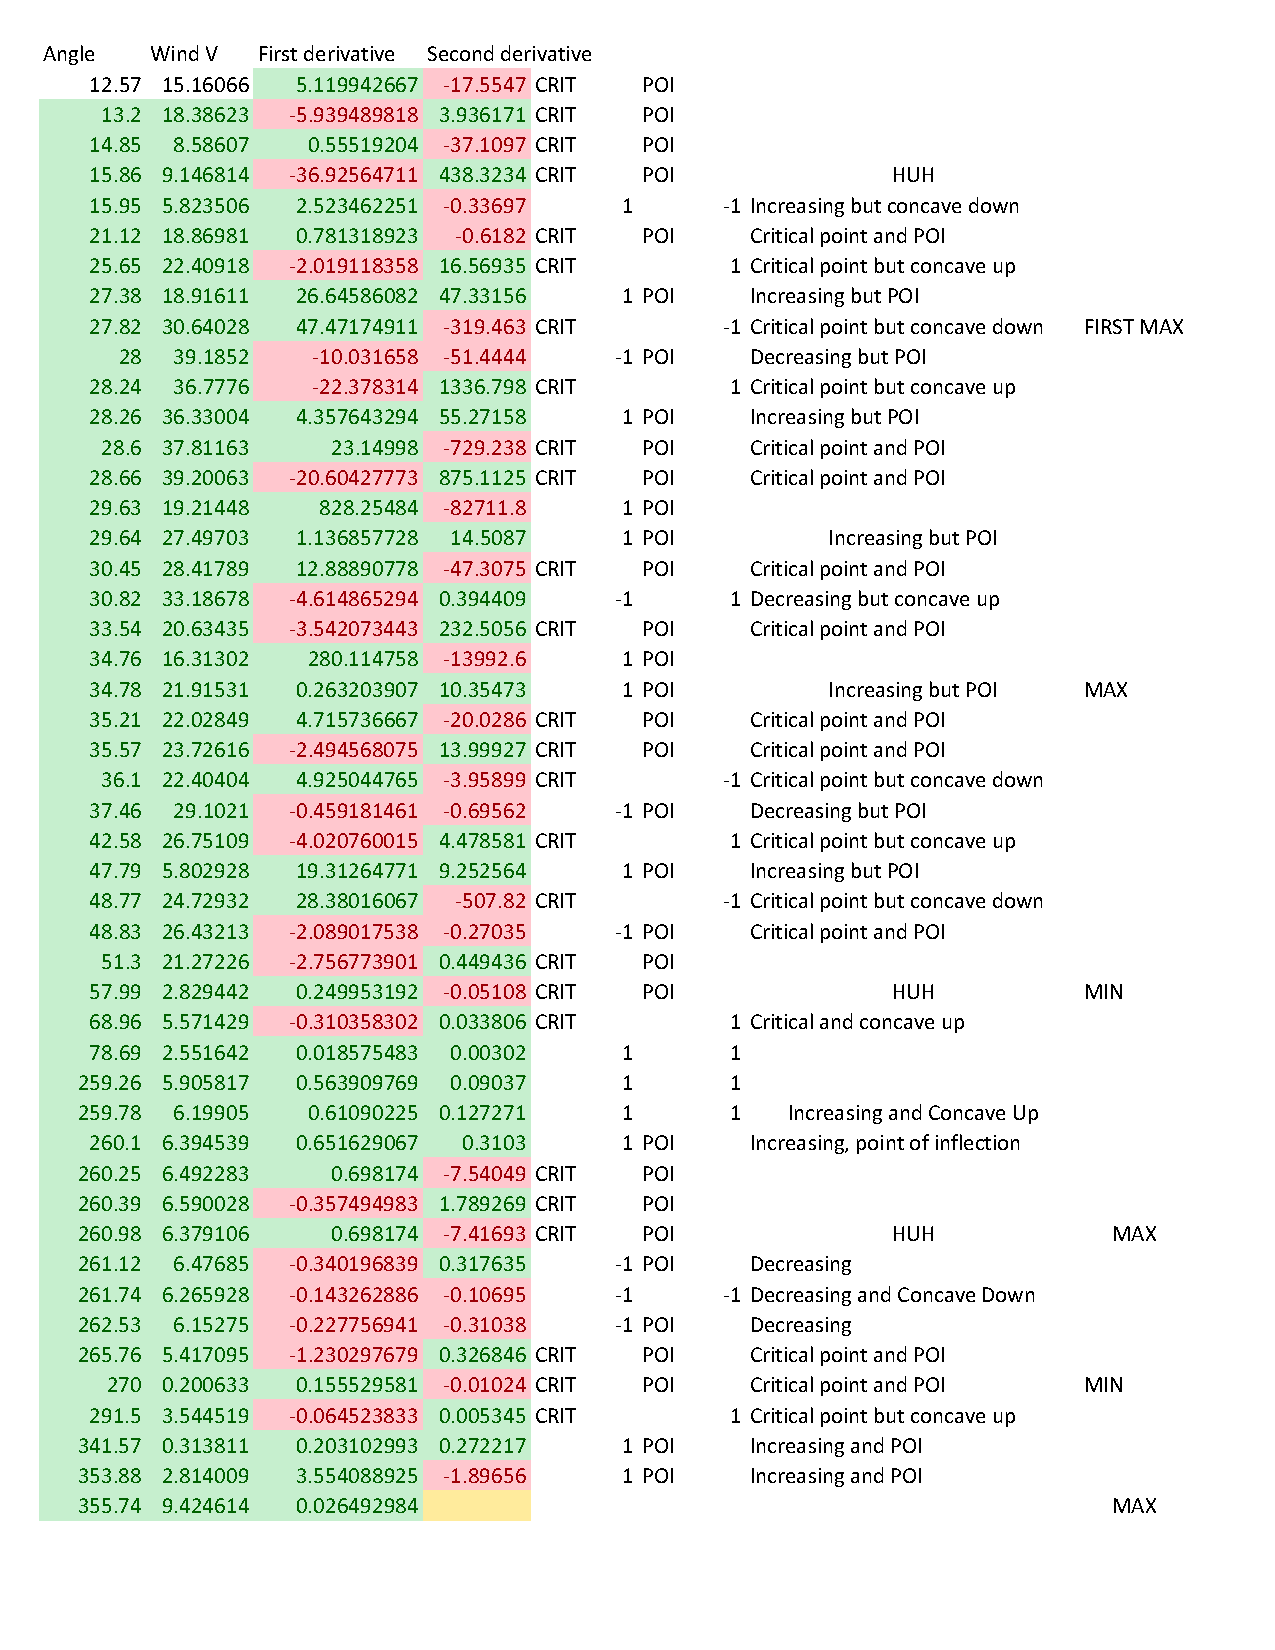
\includegraphics[width=\textwidth]{alan-data-3.pdf}
\caption{Numerical Analysis of Wind Velocity vs. Wind Angle. \\Note: Critical points on this spreadsheet are where the first derivative changes sign. Points of inflection on this spreadsheet are where the second derivative changes sign. This is as the Intermediate Value Theorem requires that at some point between the points the derivative be ACTUALLY equal to zero, creating either a critical point or point of inflection.}
\end{table}

\begin{table}
\centering
\caption{Raw Data From Predictions of Wind Speed Vs. Height}
\label{joshtable1}
\begin{tabular}{@{}llllll@{}}
\toprule
altitude (m) & wind speed (m/s) & first derivative & second    & f is & concave \\ \midrule
947.84       & 5.90581712       &                  &           &      &         \\
985.55       & 6.1990502        & 0.007776003      &           & +    &         \\
1023.37      & 6.39453892       & 0.005168924      & -6.89E-05 & +    & DOWN    \\
1061.3       & 6.49228328       & 0.002576967      & -6.83E-05 & +    & DOWN    \\
1101.25      & 6.49228328       & 0                & -6.45E-05 & -    & DOWN    \\
1141.34      & 6.49228328       & 0                & 0         & -    & DOWN    \\
1182.52      & 6.59002764       & 0.002373588      & 5.76E-05  & +    & UP      \\
1224.81      & 6.59002764       & 0                & -5.61E-05 & -    & DOWN    \\
1268.21      & 6.59002764       & 0                & 0         & -    & DOWN    \\
1313.71      & 6.59002764       & 0                & 0         & -    & DOWN    \\
1361.33      & 6.59002764       & 0                & 0         & -    & DOWN    \\
1411.1       & 6.59002764       & 0                & 0         & -    & DOWN    \\
1463.04      & 6.49228328       & -0.001881871     & -3.62E-05 & -    & DOWN    \\
1518.18      & 6.49228328       & 0                & 3.41E-05  & -    & UP      \\
1575.56      & 6.47684996       & -0.000268967     & -4.69E-06 & -    & DOWN    \\
1639.2       & 6.47684996       & 0                & 4.23E-06  & -    & UP      \\
1710.22      & 6.3791056        & -0.001376293     & -1.94E-05 & -    & DOWN    \\
1792.78      & 6.3791056        & 0                & 1.67E-05  & -    & UP      \\
1889.17      & 6.26592792       & -0.001174164     & -1.22E-05 & -    & DOWN    \\
2000.74      & 6.26592792       & 0                & 1.05E-05  & -    & UP      \\
2130.05      & 6.15275024       & -0.000875243     & -6.77E-06 & -    & DOWN    \\
2277.72      & 5.41709532       & -0.004981749     & -2.78E-05 & -    & DOWN    \\
2447.89      & 3.54451916       & -0.01100415      & -3.54E-05 & -    & DOWN    \\
2641.95      & 2.81400868       & -0.003764354     & 3.73E-05  & -    & UP      \\
2861.54      & 5.82350608       & 0.013705075      & 7.96E-05  & +    & UP      \\
3107.44      & 9.14681432       & 0.013514877      & -7.73E-07 & +    & DOWN    \\
3381.51      & 15.16066468      & 0.021942753      & 3.08E-05  & +    & UP      \\
3681.25      & 18.38622856      & 0.010761206      & -3.73E-05 & +    & DOWN    \\
4002.43      & 18.86980592      & 0.001505627      & -2.88E-05 & +    & DOWN    \\ \bottomrule
\end{tabular}
\end{table}


\begin{table}
\centering
\caption{Table \ref{joshtable1} Continued}
\label{joshtable2}
\begin{tabular}{@{}llllll@{}}
\toprule
altitude (m) & wind speed (m/s) & first derivative & second    & f is & concave \\ \midrule
4344.09      & 18.91610588      & 0.000135515      & -4.01E-06 & +    & DOWN    \\
4706.73      & 19.2144834       & 0.000822793      & 1.90E-06  & +    & UP      \\
5089.27      & 20.63434884      & 0.003711678      & 7.55E-06  & +    & UP      \\
5491.59      & 22.02849208      & 0.00346526       & -6.12E-07 & +    & DOWN    \\
5913.8       & 21.9153144       & -0.00026806      & -8.84E-06 & -    & DOWN    \\
6358.13      & 23.72615728      & 0.004075446      & 9.78E-06  & +    & UP      \\
6822.71      & 26.43213272      & 0.005824563      & 3.76E-06  & +    & UP      \\
7313.41      & 24.72932308      & -0.003470164     & -1.89E-05 & -    & DOWN    \\
7830.24      & 26.751088        & 0.003911857      & 1.43E-05  & +    & UP      \\
8382.36      & 29.10209708      & 0.004258149      & 6.27E-07  & +    & UP      \\
8972.84      & 33.18678244      & 0.006917568      & 4.50E-06  & +    & UP      \\
9591.32      & 36.33003528      & 0.005082222      & -2.97E-06 & +    & DOWN    \\
10215.39     & 37.811634        & 0.002374091      & -4.34E-06 & +    & DOWN    \\
10824.28     & 39.2006328       & 0.002281198      & -1.53E-07 & +    & DOWN    \\
11416.76     & 39.18519948      & -2.60E-05        & -3.89E-06 & -    & DOWN    \\
11995.67     & 36.77760156      & -0.004158847     & -7.14E-06 & -    & DOWN    \\
12565.71     & 30.64028464      & -0.010766467     & -1.16E-05 & -    & DOWN    \\
13130.59     & 28.41788656      & -0.003934284     & 1.21E-05  & -    & UP      \\
13704.45     & 27.4970318       & -0.001604668     & 4.06E-06  & -    & UP      \\
14307.19     & 22.40918064      & -0.008441204     & -1.13E-05 & -    & DOWN    \\
14949.59     & 16.31301924      & -0.009489666     & -1.63E-06 & -    & DOWN    \\
15626.44     & 21.2722594       & 0.007326941      & 2.48E-05  & +    & UP      \\
16364.28     & 22.4040362       & 0.001533905      & -7.85E-06 & +    & DOWN    \\
17178.71     & 9.42461408       & -0.015936817     & -2.15E-05 & -    & DOWN    \\
18095.86     & 5.80292832       & -0.003948848     & 1.31E-05  & -    & UP      \\
19133.84     & 5.57142852       & -0.000223029     & 3.59E-06  & -    & UP      \\
20359.21     & 2.829442         & -0.00223768      & -1.64E-06 & -    & DOWN    \\
21888.32     & 2.55164224       & -0.000181674     & 1.34E-06  & -    & UP      \\
23904.7      & 0.20063316       & -0.001165955     & -4.88E-07 & -    & DOWN    \\
26910.97     & 0.31381084       & 3.76E-05         & 4.00E-07  & +    & UP      \\
33038.6      & 8.58607036       & 0.001349993      & 2.14E-07  & +    & UP      \\
AVG:         & 14.57059741      & 0.000699214      & -3.47E-06 & +    & DOWN    \\ \bottomrule
\end{tabular}
\end{table}


\begin{table}
\centering
\caption{Set of parameters for fitting 20th degree polynomial}
\label{nathantable1}
\begin{tabular}{@{}l@{}}
\toprule
Final set of parameters            Asymptotic Standard Error     \\ \midrule
=======================            ==========================    \\
a               = -6.67852e+009    +/- 1.669e+009   (24.98\%) 20 \\
b               = 6.32378e+010     +/- 1.577e+010   (24.94\%) 19 \\
c               = -2.66395e+011    +/- 6.633e+010   (24.9\%) 18  \\
d               = 6.47242e+011     +/- 1.605e+011   (24.8\%) 17  \\
e               = -9.63695e+011    +/- 2.362e+011   (24.51\%) 16 \\
f               = 7.92962e+011     +/- 1.855e+011   (23.4\%) 15  \\
g               = -3.20871e+010    +/- 5.495e+010   (171.2\%) 14 \\
h               = -8.46881e+011    +/- 2.742e+011   (32.37\%) 13 \\
i               = 1.25703e+012     +/- 3.871e+011   (30.8\%) 12  \\
j               = -1.08047e+012    +/- 3.361e+011   (31.11\%) 11 \\
k               = 6.42917e+011     +/- 2.063e+011   (32.08\%) 10 \\
l               = -2.78471e+011    +/- 9.343e+010   (33.55\%) 9  \\
m               = 8.91538e+010     +/- 3.165e+010   (35.5\%) 8   \\
n               = -2.10955e+010    +/- 8.004e+009   (37.94\%) 7  \\
o               = 3.65601e+009     +/- 1.492e+009   (40.8\%) 6   \\
p               = -4.57416e+008    +/- 2e+008       (43.73\%) 5  \\
q               = 4.06564e+007     +/- 1.858e+007   (45.71\%) 4  \\
r               = -2.53831e+006    +/- 1.129e+006   (44.48\%) 3  \\
s               = 111081           +/- 4.087e+004   (36.79\%) 2  \\
t               = -3311.86         +/- 747.2        (22.56\%) 1  \\
u               = 266.925          +/- 4.736        (1.774\%) c  \\ \bottomrule
\end{tabular}
\end{table}

\begin{table}
\centering
\caption{}
\label{nathantable2}
\begin{tabular}{@{}ll@{}}
\toprule
First Derivative               &  \\ \midrule
A -13357E11 $\sim$ 19          &  \\
B 1.201503E12 $\sim$ 18        &  \\
C -4.795502E12 $\sim$ 17       &  \\
D 1.100308E13 $\sim$ 16        &  \\
E -1.541904E13 $\sim$ 15       &  \\
F -2.82155871931E22 $\sim$ 14  &  \\
G -4.49218E11 $\sim$ 13        &  \\
H -1.100944E13 $\sim$ 12       &  \\
I 1.5084E13 $\sim$ 11          &  \\
J -1.18844E13 $\sim$ 10        &  \\
K 6.4291E12 $\sim$ 9           &  \\
L -2.50623E12 $\sim$ 8         &  \\
M 7.132304E11 $\sim$ 7         &  \\
N -1.476685E11 $\sim$ 6        &  \\
O 2.1936E10 $\sim$ 5           &  \\
P -2.2870E9 $\sim$ 4           &  \\
Q 1.6262E8 $\sim$ 3            &  \\
R -7.6149E6 $\sim$ 2           &  \\
S 2.22162E5 $\sim$ 1           &  \\
T -3.31186E3                   &  \\
                               &  \\
Second Derivative              &  \\ \midrule
A -2.53783E12 $\sim$ 18        &  \\
B 2.1627054E13 $\sim$ 17       &  \\
C -8.151534E13 $\sim$ 16       &  \\
D 1.7604928E14 $\sim$15        &  \\
E -2.312856E14 $\sim$ 14       &  \\
F -3.95018220703E23 $\sim$ 13  &  \\
G -5.839834E12 $\sim$ 12       &  \\
H -1.3211328E14 $\sim$ 11      &  \\
I 1.65924E14 $\sim$ 10         &  \\
J -1.18844E14 $\sim$ 9         &  \\
K 5.78619E13 $\sim$ 8          &  \\
L -2.004984E13 $\sim$ 7        &  \\
M 4.9926128E12 $\sim$ 6        &  \\
N -8.86011E11 $\sim$ 5         &  \\
O 1.0968E11 $\sim$ 4           &  \\
P -9.1482E9 $\sim$ 3           &  \\
Q 4.87872E8 $\sim$ 2           &  \\
R -1.52298E7 $\sim$ 1          &  \\
S 2.22162E5                    &  \\
First Derivative X Candidates  &  \\
X = -2.91710832459E1           &  \\
X = -4.86017676428E-1          &  \\
X = -2.71992314617E-2          &  \\
Second Derivative X Candidates &  \\
X = -1.7144540973E2            &  \\
X = 3.31412357739E-2           &  \\ \bottomrule
\end{tabular}
\end{table}

\end{document}
